\documentclass[11pt,a4paper,twoside,openright]{report}

\usepackage[english]{ETHDAsfs}
\usepackage{amsbsy}
\usepackage{amssymb}
\usepackage{graphicx}
\usepackage[longnamesfirst]{natbib}
\usepackage{texab}
%\usepackage{mathrsfs}
\usepackage{enumerate}
\usepackage{relsize}
\usepackage{color} 
\usepackage[cmex10]{amsmath}
\usepackage{amsfonts}
\usepackage{savesym}
\usepackage{epstopdf}
\savesymbol{IF}
\usepackage{algorithmic}
\usepackage[center]{caption}
\usepackage{pstool}
\usepackage[usenames,dvipsnames]{xcolor}
\usepackage{easybmat}
\usepackage{hyperref} 
\definecolor{Mygrey}{gray}{0.75}
%%----------------------------------------------------------------------------

%%------- Theoreme ---
\newtheorem{definition}{Definition}[subsection]
\newtheorem{lemma}[definition]{Lemma}
\newtheorem{theorem}[definition]{Theorem}
\newtheorem{Coro}[definition]{Corollary}
\theoremstyle{definition} 
\newtheorem{example}[definition]{Example}
\newtheorem{proposition}{Proposition}
\newtheorem*{note}{Note}
\newtheorem*{remark}{Remark}

\DeclareMathOperator*{\plim}{plim}
\DeclareMathOperator{\Tr}{Tr}
% \def\MR#1{\href{http://www.ams.org/mathscinet-getitem?mr=#1}{MR#1}}

%% custom macros
\newcommand{\state}{\mathbf{s}} % used to denote the system states
\newcommand{\sysInput}{\mathbf{u}} % used to denote the system inputs
\newcommand{\context}{\mathbf{c}} % used to denote contexts
\newcommand{\observations}{\mathbf{y}} % used for the observed output
\newcommand{\aatop}[2]{\genfrac{}{}{0pt}{}{#1}{#2}}
\newcommand{\defeq}{\mathrel{\mathop:}=}
%\renewcommand{\theequation}{\arabic{equation}}
\numberwithin{equation}{chapter}

%%%%%%%%%%%%%%%%%%%%%%%%%%%%%%%%%%%%%%%%%%%%%%%%%
%%% Path for your figures
%%%%%%%%%%%%%%%%%%%%%%%%%%%%%%%%%%%%%%%%%%%%%%%%%
% Set the paths where all figures are taken from:
\graphicspath{{Pictures/}}

%%%%%%%%%%%%%%%%%%%%%%%%%%%%%%%%%%%%%%%%%%%%%%%%%
%%% Define your own commands here
%%%%%%%%%%%%%%%%%%%%%%%%%%%%%%%%%%%%%%%%%%%%%%%%%
\newcommand{\Bruch}[2]{{}^{#1}\!\!/\!_{#2}}
\renewcommand{\labelenumi}{\roman{enumi}.)}


\begin{document}
\bibliographystyle{plain}

\pagenumbering{roman}%- roman numbering for first few pages

%%%%%%%%%%%%%%%%%%%%%%%%%%%%%%%%%%%%%%%%%%%%%%%%%
%%% Title page
%%%%%%%%%%%%%%%%%%%%%%%%%%%%%%%%%%%%%%%%%%%%%%%%%
\period{Spring 2013}
\dasatype{Master Thesis}
\students{Okan Ko\c c}
\mainreaderprefix{Advisor:}
\mainreader{Prof.\ Hans Rudolf K\" unsch}
\alternatereaderprefix{Co-Advisor}
\alternatereader{Prof.\ Raffaello D'Andrea}
\submissiondate{March 10th 2013}
\title{Gaussian Process \\ Optimization based Learning \\ for Trajectory Tracking}

\maketitle
\cleardoublepage
 %%~~~~~~~~~~~~~~~~~~~~~~~~~~~~~~~~~~~~~~~~

%%%%%%%%%%%%%%%%%%%%%%%%%%%%%%%%%%%%%%%%%%%%%%%%%
%%% Insert here acknowledgements and abstract
%%%%%%%%%%%%%%%%%%%%%%%%%%%%%%%%%%%%%%%%%%%%%%%%%
%% Dedication (optional)
\markright{}
\vspace*{\stretch{1}}
\begin{center}
    zum Wohl!
\end{center}
\vspace*{\stretch{2}}

% Abstract should not be longer than one page.
\newpage
\markboth{Abstract}{Abstract}
\chapter*{Abstract}

Short summary of my thesis.
 

%%% Local Variables: 
%%% mode: latex
%%% TeX-master: "MasterThesisSfS"
%%% End: 


%%%%%%%%%%%%%%%%%%%%%%%%%%%%%%%%%%%%%%%%%%%%%%%%%
%%% Table of contents and list of figures and 
%%% tables (no need to change this usually)
%%%%%%%%%%%%%%%%%%%%%%%%%%%%%%%%%%%%%%%%%%%%%%%%%
\newpage
\tableofcontents
\newpage
\listoffigures
\newpage
\listoftables

%% Notations and glossary (optional)
\cleardoublepage
\phantomsection
\addcontentsline{toc}{chapter}{\protect\numberline{}{Notation}}
\markboth{Notation}{Notation}
\chapter*{Notation}
% add notation for CGP-UCB, i.e. mu kernel, beta ...

\section*{Symbols}

\begin{tabular}{ll}
$\state$ & state \\
$\sysInput$ & control input \\
$\context$ & context \\
$x$ & contexts and actions combined \\
$N$ & number of data samples \\
$J$ & total cost function \\
$J_{t}$ & stage cost at time $t$ \\
$\beta_{t}$ & exploration-exploitation parameter at time $t$ \\
$\mathbf{b}$ & mean hyperparameters of a Gaussian Process \\
$\boldsymbol{\theta}$ & covariance hyperparameters of a Gaussian Process \\
\end{tabular}

\section*{Acronyms and Abbreviations}

\begin{tabular}{ll}
\textbf{GP}      & Gaussian Process \\
\textbf{ILC}     & Iterative Learning Control \\
\textbf{MPC}     & Model Predictive Control (or Receding Horizon Control) \\
\textbf{DP}      & Dynamic Programming \\
\textbf{UCB}     & Upper Confidence Bound \\
\textbf{CGP-UCB} & Contextual Gaussian Process based Upper Confidence Bound optimization \\
\textbf{ML}      & Maximum Likelihood Estimation \\
\textbf{REML}    & Restricted Maximum Likelihood Estimation \\
\textbf{RKHS} 	 & Reproducing Kernel Hilbert Space \\
\textbf{HJB}     & Hamilton Jacobi Bellman equation \\
\textbf{GLS} 	 & Generalized Least Squares \\
\textbf{SSE} 	 & Sum of Squares Error \\
\textbf{CG}      & Conjugate Gradient Algorithm 
\end{tabular}

\cleardoublepage
\pagenumbering{arabic}%--- switch back to standard numbering 

%%%%%%%%%%%%%%%%%%%%%%%%%%%%%%%%%%%%%%%%%%%%%%%%%
%%% Main text... 
%%%%%%%%%%%%%%%%%%%%%%%%%%%%%%%%%%%%%%%%%%%%%%%%%
\setcounter{chapter}{-1}
\chapter{Introduction} 

Description of the work. Prepare the reader for the following chapters.

You will cite litterature here, typically

%%% Local Variables: 
%%% mode: latex
%%% TeX-master: "MasterThesisSfS"
%%% End: 

\chapter{First Chapter} 

\section{To include a picture}
\begin{figure}[hbt!]%--- Picture 'H'ere, 'B'ottom or 'T'op; '!' Try to
                    %impose your will to LaTeX
  \epsfCfile{.85}{geys-2kern} %<< no file extension
  %%         --- .85 stands for 85% of text width
  \caption[Geyser data: binned histogram, Silverman's and another
  kernel]%<<-- Legend for the list of figures at the beginning of you thesis
  {Old Faithful Geyser eruption lengths, $n=272$; binned data and two
    (Gaussian) kernel density estimates ($\times 10$) with $h=h^*= .3348$
    and $h= .1$ (dotted).}% legend displayed below the graph.
  \label{fig:geys1}
\end{figure}

Or also with \texttt{includegraphics}:
\begin{figure}[hbt!]%--- Picture 'H'ere, 'B'ottom or 'T'op; '!' Try to
                    %impose your will to LaTeX
  \centering
  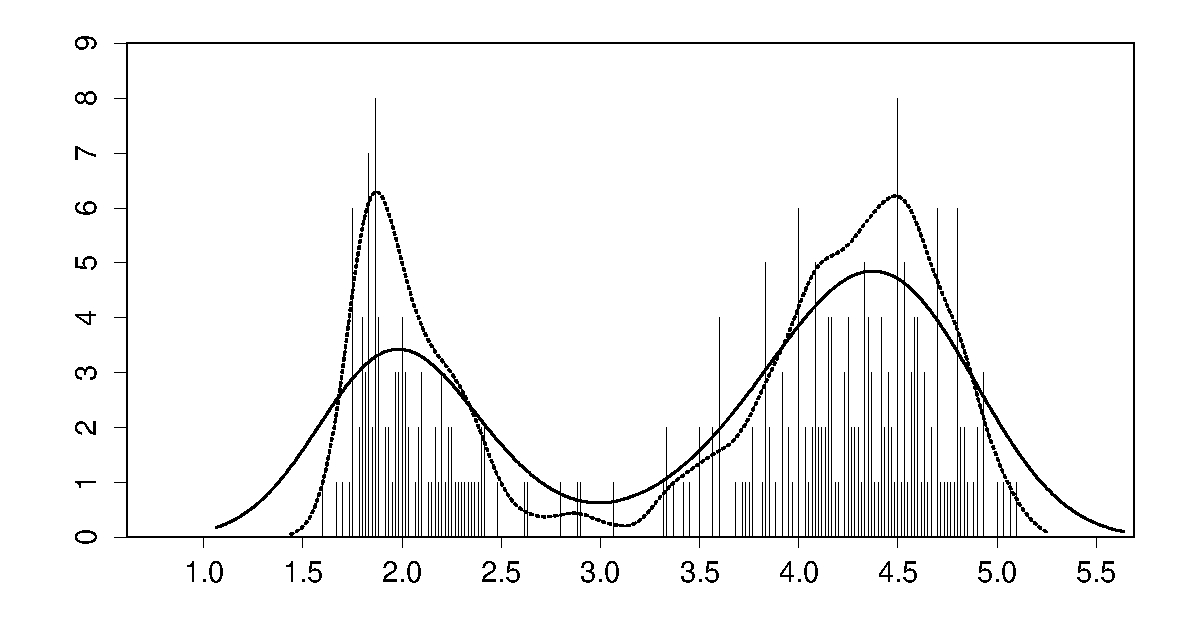
\includegraphics[width=.5\textwidth]{geys-2kern} %<< no file extension
  %%         --- .5\textwidth stands for 50% of text width
  \caption[Geyser data: binned histogram, Silverman's and another
  kernel]%<<-- Legend for the list of figures at the beginning of you thesis
  {Old Faithful Geyser eruption lengths, $n=272$; binned data and two
    (Gaussian) kernel density estimates ($\times 10$) with $h=h^*= .3348$
    and $h= .1$ (dotted).}% legend displayed below the graph.
  \label{fig:geys2}
\end{figure}

\section{To make a proof}
\begin{proof}
  $1 + 1 = 2$
\end{proof}

\section{To include \Rp code}
See information in Appendix~\ref{app:complement}.


\section{Other information}
Put a text between quotes: make sure to use nice quotes, such as ``quote''.

Cite a document in the bibliography (an example here): \cite{Reference}.
%%--> in file   myReferences.bib  (same directory)
Or mention that \citeauthor{HamF85} (a person) or \citeauthor{StaWW91} (two
persons) have already done quite a bit work.

Referencing a different part of your work: please refer to Appendix \ref{app:complement}.


%%% Local Variables: 
%%% mode: latex
%%% TeX-master: "MasterThesisSfS"
%%% End: 

\chapter{Hyperparameter Estimation}
\label{Chapter2}

\section{Maximum Likelihood Estimation}

In Bayesian inference, ideally, given noisy observations $\observations = \{y_1,\ldots,y_N\}$ from data samples $X = \{x_1,\ldots,x_N\}$, we would like to predict the posterior distribution of unknown test points $\mathbf{x}^{*}$:

\begin{equation}
p(\observations^{*}|\mathbf{x}^{*},\observations,X,\mathcal{H}_{i}) = \int p(\observations^{*}|\mathbf{x}^{*},\observations,X,\theta,\mathcal{H}_{i}) p(\theta|X,\observations,\mathcal{H}_{i})d\theta \label{posteriorInf} 
\end{equation}

where $\mathcal{H}_i$ denotes the $i$'th model structure and $\theta$ are the hyperparameters of this model. $p(\observations^{*}|\mathbf{x}^{*},\observations,X,\theta,\mathcal{H}_{i}) = \mathcal{N}(\mu_{\theta}, K_{\theta})$ calculated according to the Gaussian Process, e.g. $K_{\theta} = [k(x,x')]_{x,x' \in \mathbf{x}^{*}}$ is the covariance matrix calculated using $\mathcal{H}_{i}$ and $\theta$ from the update equations, \eqref{gpUpdate_mu} and \eqref{gpUpdate_sigma}. To compute \eqref{posteriorInf} then, we need the quantity $p(\theta|X,\observations,\mathcal{H}_{i})$:

\begin{align}
p(\theta|X,\observations,\mathcal{H}_{i})) &= \frac{p(\observations|X,\theta,\mathcal{H}_{i})p(\theta|\mathcal{H}_{i})}{p(\observations|X,\mathcal{H}_{i})} \label{posteriorTheta} \\
&= \frac{p(\observations|X,\theta,\mathcal{H}_{i})p(\theta|\mathcal{H}_{i})}{\int p(\observations|X,\theta,\mathcal{H}_{i}) p(\theta|\mathcal{H}_{i})d\theta} \label{evidence}
\end{align}

Unfortunately, the integral in \eqref{evidence}, also known as the \emph{evidence} is generally not tractable, especially when there are several hyperparameters to marginalize over, so one has to resort to approximate inference methods, such as Markov-Chain Monte Carlo (MCMC). Assuming the distribution $p(\theta|X,\observations,\mathcal{H}_{i}))$ is sharply peaked\footnote{Otherwise, it will underestimate the variance of the predictive distribution.} however, as a widely used approximation one can maximize the log likelihood for the hyperparameters:

\begin{equation}
\hat{\theta}_{ML} = \argmax_{\theta} \log p(\observations|X,\theta,\mathcal{H}_{i}) \label{MLE}
\end{equation}

In this case the predictive distribution will be $p(\observations^{*}|\mathbf{x}^{*},\observations,X,\mathcal{H}_{i}) \approx  p(\observations^{*}|\mathbf{x}^{*},\observations,X,\hat{\theta}_{ML},\mathcal{H}_{i})$. \\

The likelihood function $p(\observations|X,\theta,\mathcal{H}_{i})$ is called the \emph{marginal likelihood} in \cite{GPbook} because it is the denominator in the posterior for a parametric model:

\begin{equation}
p(\mathbf{w}|\observations,X,\theta,\mathcal{H}_{i}) = \frac{p(\observations|X,\mathbf{w}, \mathcal{H}_{i})p(\mathbf{w}|\theta,\mathcal{H}_{i})}{p(\observations|X,\theta,\mathcal{H}_{i})} \label{parametricBayes}
\end{equation}

where $\mathbf{w}$ are the parameters corresponding to the basis functions. They are marginalized over in the likelihood function:

\begin{equation}
p(\observations|X,\theta,\mathcal{H}_{i}) = \int p(\observations|X,\mathbf{w},\mathcal{H}_{i})p(\mathbf{w}|\theta,\mathcal{H}_{i})d\mathbf{w} \label{lvl2int}
\end{equation}

This integral, unlike the integral in \eqref{evidence} is tractable because the distributions in the integrand are both Gaussian distributed. Equivalently, from a Gaussian Process point of view, $\observations$ values are drawn from a Gaussian multivariate distribution, so the negative log likelihood can be written as:

\begin{align}
\textbf{nll} &= - \log \frac{1}{(2\pi^{N/2})|K_{\theta}|^{1/2}}e^{-(\observations - \mathbf{\mu})^{\mathrm{T}}K_{\theta}^{-1}(\observations - \mathbf{\mu})} \\
&= \frac{N}{2}\log(2\pi) + \underbrace{\frac{1}{2}\log|K_{\theta}|}_{\text{complexity penalty}} + \underbrace{(\observations - \mathbf{\mu})^{\mathrm{T}}K_{\theta}^{-1}(\observations - \mathbf{\mu})}_{\text{data fit}}
\label{nll}
\end{align}

Maximizing the likelihood is equivalent to minimizing the log likelihood given in \eqref{nll}. The negative log likelihood (nll), aside from the first constant term, is composed of two complementary parts: the data fit term and the complexity penalty term. The complexity penalty term eliminates more complicated models that are able to explain the data well and prefers simpler models. 

\subsection*{RHKS norm}
% add more after reading Wahba
The data fit term also corresponds to the squared RKHS-norm $\observations^{\mathrm{T}}K_{\theta}^{-1}\observations$ of a zero mean function $\observations(t)$ corrupted with Gaussian white noise. The value of the squared RKHS-norm can be acquired from the minimized negative log likelihood and then used as a good estimate for a bound $B$ for CGP-UCB optimization, assuming that the function to be optimized is smooth enough between the data points $X$\footnote{otherwise the bound $B$ might be a too low estimate for $||y||_{\mathrm{K_\theta}}$}. This bound is used to set the $\beta_t$ parameter that balances exploration-exploitation in the RKHS version of CGP-UCB optimization. More precisely, its value is given in Theorem 3 in \cite{Krause1} as follows:

\begin{equation}
\beta_{t} = 2B + 300 \gamma_t \log^{3}(t/\delta) \label{Thm3KrauseBeta}
\end{equation}

where $\delta$ is the constant controlling the probability of convergence of (cumulative) regret. The \emph{maximum information gain} quantity appearing in \eqref{Thm3KrauseBeta}, $\gamma_{T}$, after $T$ rounds is defined as:

\begin{equation}
\gamma_{T} \defeq \max_{X \subset D: |X|=T} \mathcal{I}(\observations_{T}; \mathbf{f}_{T}) \label{maxInfoGain}
\end{equation}

Here $\mathbf{f}_{T}$ is the latent function at the points $X$, and $\mathcal{I}(\observations_{T}; \mathbf{f}_{T}) = H(\observations_{T}) - H(\observations_{T}|\mathbf{f}_{T})$ is quantifying the reduction in uncertainty of $\mathbf{f}$ after revealing $\observations_{T}$ at $X$. For a Gaussian distribution:

\begin{equation}
\mathcal{I}(\observations_{T}; \mathbf{f}_{T}) = \frac{1}{2}\log|2\pi e K_{T}| -  \frac{1}{2}\log|2\pi e \sigma_{n}^{2}I| = \frac{1}{2}\log|I + \sigma_{n}^{-2} K_{T}|
\end{equation}

% reference needed for NP-hard
Computing the maximum information gain $\gamma_{T}$ for arbitrary $X$ is a NP-hard combinatorial optimization problem. However it can be upper-bounded by a greedy procedure: pick at each step a point where the uncertainty is greatest. That is,

\begin{equation}
x_{t} = \argmax_{x \in D} \sigma_{t-1}(x)
\end{equation}

The information gain that is achieved after $T$ rounds using this method, denoted by $F_{T}$, can upper-bound $\gamma_{T}$:

\begin{equation}
\frac{F_{T}}{1 - 1/e} \geq \gamma_{T} \label{maxInfoGainUppBnd}
\end{equation}

The inequality \eqref{maxInfoGainUppBnd} is very useful because $\gamma_{T}$ appears in the regret achieved by CGP-UCB after $T$ rounds. Precisely:

\begin{equation}
\Pr \lbrace R_{T} \leq \sqrt{C_{1}T\beta_{T}\gamma_{T}} \rbrace \geq 1 - \delta \label{Thm3KrauseRegretBnd}
\end{equation}

where $C_{1} = \frac{8}{\log(1 + \sigma_{n}^{-2})}$. Using \eqref{maxInfoGainUppBnd}, one can show (probabilistic) sublinear regret for \eqref{Thm3KrauseRegretBnd}.

\subsection*{Implementation}
% talk about profile likelihood

The negative log likelihood minimization is generally performed in the literature using derivative-based methods, such as gradient descent or conjugate gradients (CG). The gradient of the log likelihood in \eqref{nll} can be calculated and fed to the algorithm to speed up the process, or the gradient can be approximated numerically. See Rasmussen's GP Toolbox \cite{GPML}, for an implementation using a conjugate gradient approach. Profile likelihood estimation, which tries to estimate (aside from $l$) only a scaled $\sigma_n / \sigma_s$ noise parameter, reduces the number of independent parameters by 1 and may yield more accurate estimates for length-scale parameters $l$.

\subsection{Restricted Maximum Likelihood}
% put references

Maximum likelihood (ML) will perform poorly in cases where the mean component of the GP affects the observations. ML usually will try to compensate for the mean component by considering covariance parameter values that may be far off. In such cases, using restricted maximum likelihood (REML) may be a better option. 

The restricted maximum likelihood method finds a linear transformation on observations $\observations$ such that the resulting vector does not involve the fixed effect parameter vector $\mathbf{b}$ regardless of their values. These linear combinations are the residuals obtained after a generalized least squares regression on the fixed effects. The fixed effects in the case of a Gaussian Process hyperparameter estimation are the mean function parameters:

\begin{equation}
\mu(x) = b_{0} + b_{1:n}^{\mathrm{T}}x \label{mean}
\end{equation}

Modifying the design matrix $X$ as 
$\bar{X} = 
\left(
\begin{array}{ccc}
\mathbf{1}^{\mathrm{T}} \\
X^{\mathrm{T}}
\end{array}
\right)^{\mathrm{T}}$
and performing generalized least squares (GLS) on the mean parameters $\mathbf{b}$ at the $n$'th step of ML optimization:

\begin{equation}
\tilde{\mathbf{b}}_{n} = (\bar{X}^{\mathrm{T}}K_{\theta_{n}}^{-1}\bar{X})^{-1}\bar{X}^{\mathrm{T}}K_{\theta_{n}}^{-1}\observations \label{GLS}
\end{equation}

one can do (full) Maximum Likelihood Estimation on the residuals $\hat{\observations}$ to get the REML estimates:

\begin{align}
\textbf{nll}_{\observations_{n}} &= - \log \frac{1}{(2\pi^{(N-r)/2})|\hat{K}_{\theta}|^{1/2}}e^{-\hat{\observations}_{n}^{\mathrm{T}}\hat{K}_{\theta}^{-1}\hat{\observations}_{n}} \\
&= \frac{N-r}{2}\log(2\pi) + \frac{1}{2}\log|\hat{K}_{\theta}| + \hat{\observations}_{n}^{\mathrm{T}} \hat{K}_{\theta}^{-1} \hat{\observations}_{n}
\label{nll_reml}
\end{align}

where $r = \text{rank}(X)$ and

\begin{align}
\hat{\observations}_{n} &= \observations - \bar{X}\tilde{\mathbf{b}}_{n} \\
&= \observations - \bar{X}(\bar{X}^{\mathrm{T}}K_{\theta_{n}}^{-1}\bar{X})^{-1}\bar{X}^{\mathrm{T}}K_{\theta_{n}}^{-1}\observations \\
&= \underbrace{(I -\bar{X} (\bar{X}^{\mathrm{T}}K_{\theta_{n}}^{-1}\bar{X})^{-1}\bar{X}^{\mathrm{T}}K_{\theta_{n}}^{-1})}_{\defeq R_{n}}\observations 
\end{align}

is a linear transformation of $\observations$ to the residuals. The linear transformation $R_{n}$ causes the covariance matrix $K_{\theta_{n}}$ to be transformed as follows:

\begin{equation}
\hat{K}_{\theta_{n}} = R_{n}^{\mathrm{T}}K_{\theta_{n}}R_{n}
\end{equation}

In \cite{reml} it is shown that \eqref{nll_reml} is equivalent to the following:

\begin{align}
\textbf{nll}_{\observations_{n}} &= \frac{N-r}{2}\log(2\pi) + \underbrace{\frac{1}{2}(\log|K_{\theta_{n}}| + \log|\bar{X}^{\mathrm{T}}K_{\theta_{n}}^{-1}\bar{X}|)}_{\text{complexity penalty}} + \underbrace{(\observations - \bar{X}\tilde{\mathbf{b}}_{n})^{\mathrm{T}}K_{\theta_{n}}^{-1}(\observations - \bar{X}\tilde{\mathbf{b}}_{n}))}_{\text{data fit}}
\label{nll_reml2}
\end{align}

Complexity penalty in \eqref{nll_reml2} then, is all that changes at the maximization step of an Expectation-Maximization (EM) type REML algorithm when compared to \eqref{nll}.

\subsection*{Implementation}

An EM type REML algorithm was implemented in MATLAB, after spending some time with the \emph{geoR} package in R.  Function \emph{likfit} implements REML in the geoR package but the routine is limited to 2 dimensions only and has been avoided. The custom implementation can be found in Appendix \ref{app:code}. The implementation only adds a complexity penalty and its derivative at each Maximization step to the CG optimization. The derivative term can be calculated as follows:

\begin{equation}
\frac{\partial \log |\bar{X}^{\mathrm{T}}K_{\theta}^{-1}\bar{X}|}{\partial \theta_{i}} = -\Tr \left((\bar{X}^{\mathrm{T}}K_{\theta}^{-1}\bar{X})^{-1} \bar{X}^{\mathrm{T}} K_{\theta}^{-1}\frac{\partial K_{\theta}}{\partial \theta_{i}}K_{\theta}^{-1}\bar{X} \right) \label{complexityDerivative}
\end{equation}

The sampling algorithm DIRECT could also be applied to REML to check and compare the performance of this implementation.

\section{Results}

Here we present hyperparameter estimation results using Maximum Likelihood for a 2-dimensional test case. Sample functions are drawn from zero mean and linear mean GP priors with squared exponential kernel, where the sample points form a uniform grid of $N = 100$ points between 0 and 1. An example can be seen in Figure \ref{fig:hp_test} where a GP is sampled with covariance parameters $l_x = 0.1, l_y = 0.8, \sigma_s = 1.0, \sigma_n = 0.3$ and without linear mean. It can be seen that the lower $l_x$ value causes much more variability on the $x$ dimension.

The hyperparameters are optimized with two different methods: DIRECT, a sampling-based global optimization algorithm mentioned also in \ref{Implementation}, and a conjugate-gradient (CG) based routine that also explores to reach a global minimum by random-starts. 

\begin{figure}
\center
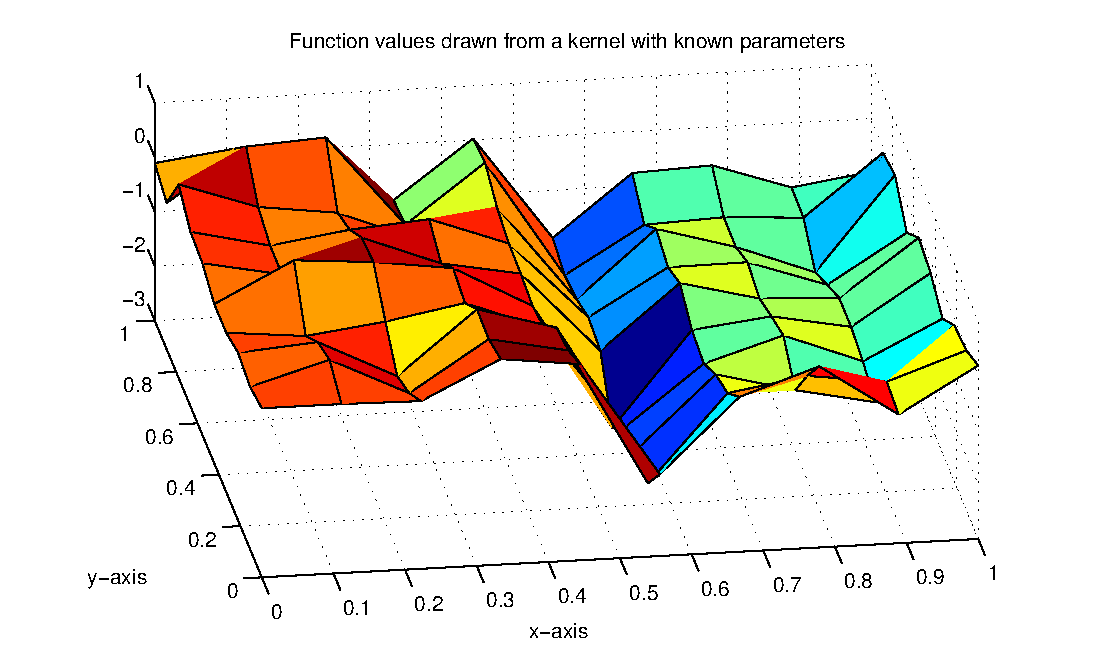
\includegraphics[scale=0.40]{test_fnc.eps}			
\caption{Zero-mean function drawn from a squared exponential kernel}
\label{fig:hp_test}
\end{figure}

The results for two sample functions are given in Tables \ref{hp_estimation1} and \ref{hp_estimation2}. Results for all functions, along with the MATLAB code can be found in Appendix \ref{app:code}. CG optimization has been started with initial values of hyperparameters set to $p_0 = 0.1$. Different sets of values for $p_0$ have also been tried, but the optimal hyperparameter estimates are always the same, due to the inherent exploration in the CG-algorithm implemented in \cite{GPML}. Estimates 1 and 2 in Tables \ref{hp_estimation1} and \ref{hp_estimation2} refer to the cases with zero mean and with linear mean, respectively.

\begin{table}
% increase table row spacing, adjust to taste
\renewcommand{\arraystretch}{1.3}
\caption{Hyperparameter estimation results - test case 1}
\label{hp_estimation1}
\centering
\scalebox{0.7}{
\begin{tabular}{ccccc}
Hyperparameters & DIRECT Estimates 1 & DIRECT Estimates 2 & CG Estimates 1 & CG Estimates 2 \\
\hline
$l_x = 0.15$      & 0.173148 & 0.173148 & 0.147529 & 0.136948 \\
$l_y = 0.50$      & 0.794753 & 0.050000 & 0.621114 & 0.591196 \\
$\sigma_s = 0.50$ & 0.681481 & 0.414815 & 0.539554 & 0.449718 \\
$\sigma_n = 0.10$ & 0.102469 & 0.122222 & 0.096381 & 0.096313 \\
$b_0 = 1.00$      & -        & 0.666667 & -        & 0.629445 \\
$b_1 = 0.50$      & -        & 1.233333 & -        & 1.460763 \\
$b_2 = -1.00$     & -        & -1.000000& -        & -1.190490  
\end{tabular}
}
\end{table}

Analyzing the results, we can easily say that the mean estimates $\mathbf{\hat{b}}$ are almost always far off. It was expected that REML would remedy the situation, but this has not been observed. In fact the implemented REML gives very close estimates to ML. However, more research needs to be done to determine how this can be improved. It seems that the number of samples $N = 100$ is not enough to accurately estimate the increased number of parameters that comes with the mean estimation. The sampling algorithm DIRECT's poor estimates of the mean parameters, even when the number of evaluations is kept very high, supports this claim. By increasing $N$, we should expect to see more accurate estimates, as a result of \emph{consistency}.

As for the covariance parameters, a slight overfitting tendency in ML can be observed in the full results given in Appendix \ref{app:code}. Overfitting underestimates the noise parameter $\sigma_n$ and overestimates the variability (i.e. $l_x, l_y$ estimates are generally lower). The overfitting effect will decrease as $N \to \infty$ as a result of the consistency of ML Estimation, but a faster convergence can be expected with a biased method. A Bayesian approach, or penalizing the hyperparameters $l$ and $\sigma_s$ might yield better results. 

\begin{table}[h!t]
% increase table row spacing, adjust to taste
\renewcommand{\arraystretch}{1.3}
\caption{Hyperparameter estimation results - test case 2}
\label{hp_estimation2}
\centering
\scalebox{0.7}{
\begin{tabular}{ccccc}
Hyperparameters & DIRECT Estimates 1 & DIRECT Estimates 2 & CG Estimates 1 & CG Estimates 2 \\
\hline
$l_x = 0.25$      & 0.277401 & 0.278704 & 0.276928 & 0.263415 \\
$l_y = 0.35$      & 0.307373 & 0.050000 & 0.307414 & 0.265768 \\
$\sigma_s = 0.40$ & 0.402743 & 0.503704 & 0.402037 & 0.318257 \\
$\sigma_n = 0.20$ & 0.180384 & 0.166667 & 0.180244 & 0.178015 \\
$b_0 = 0.40$      & -        & 0.977778 & -        & 1.004556 \\
$b_1 = 0.80$      & -        & 0.996296 & -        & 0.099169 \\
$b_2 = 0.20$      & -        & -1.000000& -        & 0.005249 
\end{tabular}
}
\end{table}

GP-optimization introduced in section \ref{Introduction} was seen to be resilient to mismatch in some hyperparameters. More precisely, mismatch in $\sigma_s$ only scales the confidence parameter $\beta_t$, whose scale was not optimized in the proofs \cite{Krause1}. It can be observed in Tables \ref{hp_estimation1} and \ref{hp_estimation2} that the noise standard deviation $\sigma_n$ is relatively well-estimated, but in case of mismatch, only the constant $C_1$ appearing in the regret bound \ref{Thm3KrauseRegretBnd} should change. Qualitatively, underestimating $\sigma_n$ corresponds in GP-optimization to unwarranted \emph{optimism} after observing $\observations$ which will cut down on the exploration. Overestimating will have the opposite effect.

The more interesting case is the mismatch in $l$ and $b_{1:n}$ parameters. In simulations, it was observed that even a slight mismatch in $b_{1:n}$ will change results drastically for the worse. Since results suggest these parameters cannot be estimated well\footnote{at least with the current sample size}, it is perhaps more proper to avoid mean parameter estimation altogether. Mismatch in $l$ parameters should also affect the results drastically. The author is currently unaware of the resilience of theoretical regret bounds that hold under general parametric mismatch, a point that deserves to be studied more in the literature.
\chapter{Summary}
\label{s:Summary}

Summarize the presented work. Why is it useful to the research field or institute?


\section{Future Work}
\label{ss:FutureWork}

Possible ways to extend the work.


%%% Local Variables: 
%%% mode: latex
%%% TeX-master: "MasterThesisSfS"
%%% End: 
 

%%%%%%%%%%%%%%%%%%%%%%%%%%%%%%%%%%%%%%%%%%%%%%%%%
%%% Bibliography                 
%%%%%%%%%%%%%%%%%%%%%%%%%%%%%%%%%%%%%%%%%%%%%%%%%
\addtocontents{toc}{\vspace{.5\baselineskip}}
\cleardoublepage
\phantomsection
\addcontentsline{toc}{chapter}{\protect\numberline{}{Bibliography}}
\bibliography{myReferences}

%%%%%%%%%%%%%%%%%%%%%%%%%%%%%%%%%%%%%%%%%%%%%%%%% 
%%% Appendices
%%%%%%%%%%%%%%%%%%%%%%%%%%%%%%%%%%%%%%%%%%%%%%%%%
\addtocontents{toc}{\vspace{.5\baselineskip}}
\appendix
\chapter{Complementary information}
\label{app:complement}

Additional material. For example long mathematical derivations could be
given in the appendix. Or you could include part of your code that is
needed in printed form. You can add several Appendices to your thesis (as
you can include several chapters in the main part of your work).

\section{Including \Rp code with verbatim}
A simple way to include code or {\it R} output is to use
\texttt{verbatim}. It just prints the text however it is (including all
spaces, ``strange'' symbols,...) in a slightly different font.
\begin{verbatim}
## loading packages
library(RBGL)
library(Rgraphviz)
library(boot)

## global variables
X_MAX <- 150

   This allows me to put as many s  p a   c es   as I want.
I can also use \ and ` and & and all the rest that is usually only 
accepted in the math mode.

I can also make as 
                  many 
             line 
    breaks as 
I want... and
             where I want. 
\end{verbatim}

\section{Including \Rp code with the \emph{listings} package}
However, it is much nicer to use the \emph{listings} package to include \Rp
code in your report. It allows you to number the lines, color the comments
differently than the code, and so on.

\lstinputlisting{Pictures/picture.R}


\section{Using Sweave to include \Rp code (and more) in your report}
The easiest (and most elegant) way to include \Rp code and its output (and
have all your figures up to date with your report) is to use Sweave. You
can find an introduction Sweave in \texttt{/u/sfs/StatSoftDoc/Sweave/Sweave-tutorial.pdf}.

%%% Local Variables: 
%%% mode: latex
%%% TeX-master: "MasterThesisSfS"
%%% End: 

\chapter{Mathematical Identities}\label{app:math}

\section{Incremental Covariance Matrix Inverse}
% note the speedup expected
% In MATLAB backslash is optimized so speedup not observed.

The GP-update equations \eqref{gpUpdate_mu} and \eqref{gpUpdate_sigma}, require the inversion of the matrix $P_{t} \defeq K(x_{T}, x_{T}) + \sigma_{n}^{2}\mathbf{I}$. Since the CPG-UCB optimization \eqref{ucb} requires $\mu(x)$ and $\sigma(x)$ at each time step $t$, this matrix needs to be inverted at each step. The backlash operation to bypass this inversion requires $N^{3}/6$ complexity. For a single test point $x_{t}$, a workaround is to use incremental inverse for the growing matrix:

\begin{equation}
P_{t+1} = 
\left(
\begin{BMAT}(rc){c:c}{c:c}
P_{t} & k(x_{T}, x_{t}) \\
k(x_{T}, x_{t})^{\mathrm{T}} & k(x_{t}, x_{t})
\end{BMAT} 
\right)
\label{CovMat}
\end{equation}

where $k(x_{T}, x_{t}) \defeq (k(x_{1}, x_{t}), \ldots, k(x_{t-1}, x_{t	}))^{\mathrm{T}}$. 

The inverse of a general invertible $n \times n$ partitioned matrix 

\begin{equation*}
A = 
\left(
\begin{array}{cc}
P & Q \\
R & S \\
\end{array} 
\right)
\end{equation*}

is the $A^{-1}$ matrix:

\begin{equation*}
A^{-1} = 
\left(
\begin{array}{cc}
\tilde{P} & \tilde{Q} \\
\tilde{R} & \tilde{S} \\
\end{array} 
\right)
\end{equation*}

where the submatrices are given as \cite{GPbook}:

\begin{eqnarray}
\tilde{P} & = & P^{-1} + P^{-1}QMRP^{-1} \label{Phat}\\
\tilde{Q} & = & -P^{-1}QM \label{Qhat} \\
\tilde{R} & = & -MRP^{-1} \label{Rhat} \\
\tilde{S} & = & M \label{Shat}
\end{eqnarray}

and $M = (S - RP^{-1}Q)^{-1}$. Applying \eqref{Phat} - \eqref{Shat} on the inverse of the covariance matrix \eqref{CovMat} we get:

\begin{equation}
P_{t+1}^{-1} = 
\left(
\begin{BMAT}(rc){c:c}{c:c}
P_{t}^{-1} + \alpha P_{t}^{-1} q_{t} q_{t}^{\mathrm{T}} P_{t}^{-1}  & -\alpha P_{t}^{-1} q_{t} \\
-\alpha q_{t}^{\mathrm{T}} P_{t}^{-1} & \alpha
\end{BMAT} 
\right)
\label{CovMatInv}
\end{equation}

where 

\begin{eqnarray}
\alpha^{-1} & = & k(x_{t}, x_{t}) - q_{t}^{\mathrm{T}}P_{t}^{-1}q_{t} + \sigma_{n}^{2} \\
q_{t} & = & k(x_{t}, x_{T})
\end{eqnarray}

$\alpha$ is a scalar that is the outcome of the last point taken, $x_{t}$. \eqref{CovMatInv} can be reached easily by plugging the block matrices in \eqref{Phat} - \eqref{Shat} and noting that the covariance matrix $P_{t}$ is square symmetric.

A practical way to iteratively compute \eqref{CovMatInv} from $P_{t}^{-1}$ would be to compute first the vector of covariances $q_{t}$  and then $q_{t}^{\mathrm{T}}P_{t}^{-1}$, and apply it throughout the block matrices in \eqref{CovMatInv}. Figure \ref{fig:runtimes} shows the results for such an implementation in MATLAB running on Intel i7 1.6 GHz Quadcore laptop, where the runtimes for the matrix multiplication operation, $(K(x_{T}, x_{T}) + \sigma_{n}^{2}\mathbf{I})^{-1}\mathbf{k}_N(x^{*})$ is compared. The incremental matrix inversion is clearly faster, especially as the data sample size $N$ increases. Figure \ref{fig:deltaruntimes} shows the effect more clearly. Note that for the backslash method, the covariance matrix is not built from scratch at each iteration, but only the last row and column are added.

\begin{figure}
\center
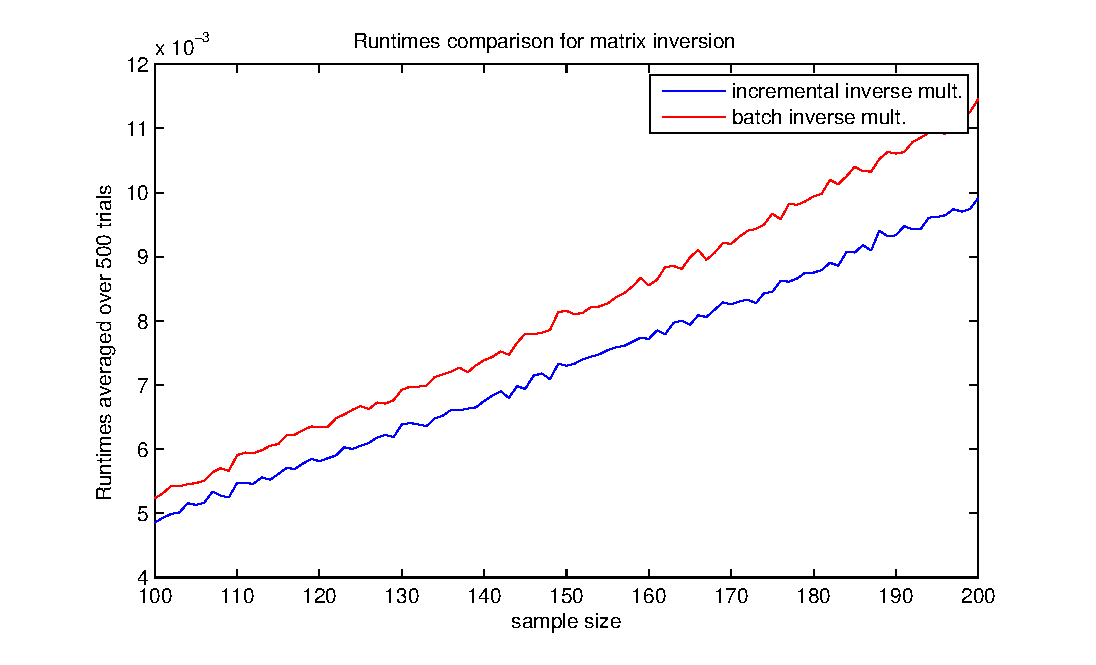
\includegraphics[scale=0.50]{runningtimes.eps}	
\caption{Runtime comparison}
\label{fig:runtimes}
\end{figure}

\begin{figure}
\center
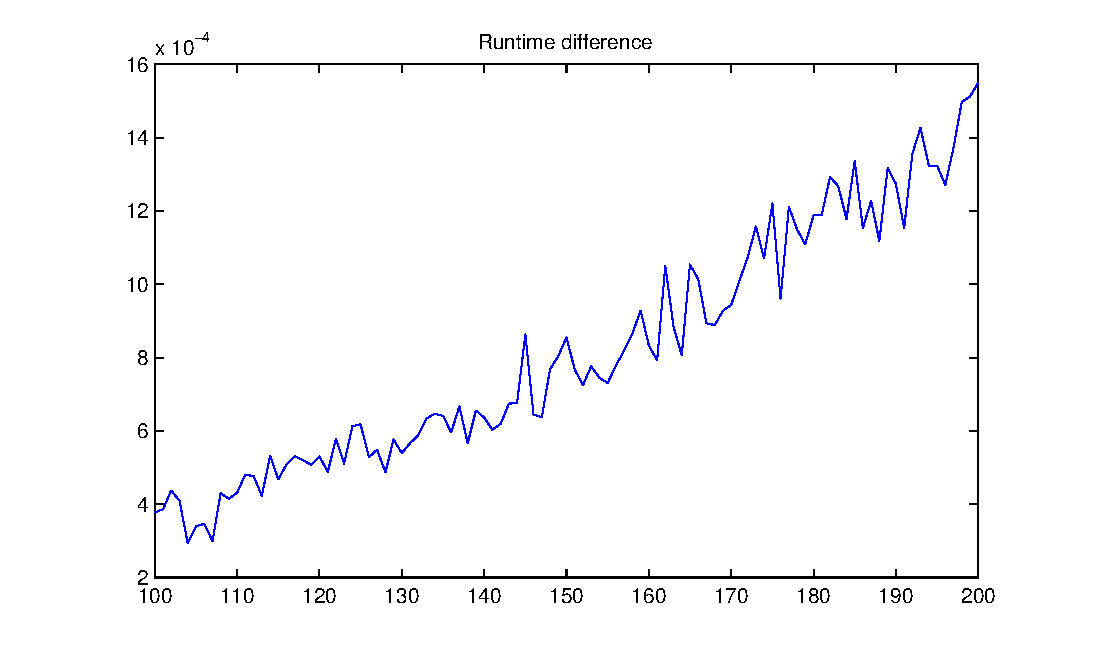
\includegraphics[scale=0.50]{delta_runningtimes.eps}	
\caption{Difference in runtimes}
\label{fig:deltaruntimes}
\end{figure}

\chapter{Trajectory Generation}\label{app:trjgen}

\section{Differential Flatness}
% read references for interesting additions
% mention Hilbert and E. Cartan ?

Differential flat systems form a subclass of nonlinear control systems, where the flatness criterion can be seen roughly as an extension of Kalman's controllability (for linear systems) to nonlinear systems \cite{Fliess95}. These \emph{flat} systems are distinguished by the fact that trajectory generation can be performed explicitly, \emph{without} integration of the differential equation.

The nonlinear control system (or the system of underdetermined ordinary differential equations):

\begin{equation}
\dot{x} = f(x, u)
\label{ODE}
\end{equation}

where $x = (x_1,\ldots, x_n)$, $u = (u_1, \ldots, u_m)$ is said to be \emph{differentially flat}\footnote{This definition is taken from Scholarpedia: \url{www.scholarpedia.org/article/Differentially\_flat\_systems}} if and only if there exist $m$ independent functions $h = (h_1, \ldots, h_m) = h(x, u, u^{(1)}, u^{(2)}, \ldots, u^{(\alpha)})$ depending on $x$ and a finite number $\alpha$ of $u$'s derivatives such that, if we set 

\begin{equation}
y = h(x, u, u^{(1)}, \ldots, u^{(\alpha)}) \label{flat}
\end{equation}

the integral curves of \eqref{ODE} satisfy for some $\beta > 0$ :

\begin{eqnarray}
x = \Gamma(y, \ldots, y^{(\beta)}) \\
u = \Lambda(y, \ldots, y^{(\beta)})
\end{eqnarray}

Once the flat (also called linearizing) output given in \eqref{flat} is determined, the path planning problem becomes particularly easy: the reference trajectory as well as the corresponding feedforward (or open-loop) control can be expressed in terms of the flat output and a finite number of its derivatives \cite{Fliess95}.

The number of flat outputs is equal to the degree of freedom of the underdetermined ordinary differential equation \eqref{ODE}, i.e. the dimension of the control input $u$.
Unfortunately, deciding if a general nonlinear control system is flat is an open problem. Many mechanical systems are known to be flat \cite{Murray97nonlinearcontrol}.

A nice and easy example for a differential flat nonlinear system (all controllable linear systems are differential flat) is the vectored thrust aircraft model borrowed from \cite{Murray97nonlinearcontrol}:

\begin{equation}
\begin{aligned}
m \ddot{x}      & = F_{1}\cos{\theta} - F_{2}\sin{\theta} \\
m \ddot{y}      & = F_{1}\sin{\theta} - F_{2}\cos{\theta} - mg \\
J \ddot{\theta} & = r F_{1} 
\end{aligned}
\label{aircraftDynamics}
\end{equation}

where $m$ is the mass of the vehicle, $J$ is the moment of inertia, and $g$ the gravitational constant. Forces acting on the vehicle consist of $F_{1}$ acting perpendicular to the axis at a distance $r$ from the center of mass, and $F_{2}$, a force parallel to the axis of the vehicle, see Figure \ref{Aircraft} from \cite{AM08}.

\begin{figure}
\center
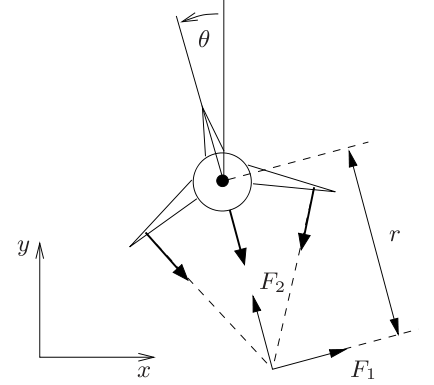
\includegraphics[scale=0.4]{aircraft.png}
\caption{Vectored thrust aircraft schematic}
\label{Aircraft}
\end{figure}

One set of flat outputs for this system is given by:

\begin{eqnarray}
z_{1} = x - (J/mr)\sin{\theta} \\
z_{2} = y + (J/mr)\cos{\theta} 
\end{eqnarray} 

Using system dynamics, the states and the control inputs $F_{1}, F_{2}$ can be found from $z_{1}$ and $z_{2}$ only. For example, $\theta$ can be found from:

\begin{equation}
\ddot{z}_{1} \cos{\theta} + (\ddot{z}_{2} + g) \sin{\theta} = 0
\end{equation}

except for the singularity $\ddot{z}_{1} = \ddot{z}_{2} + g = 0$.

See \cite{Fliess95} where the subject is introduced with \emph{dynamic feedback linearization} from a differential algebraic point of view. See \cite{Rathinam97} for a differential-geometric treatment of the subject.

\section{Splines Method}
\label{Splines}
% mention initialization, support points
% plan feasible quadrocopter trajectories (with respect to the constraints introduced) that track arbitrary user-defined shapes in the vertical plane.

In this section, we briefly summarize a method for generating feasible reference trajectories for differential flat systems under input constraints, following the spline based approach in ~\cite{ILC_Angela,Zhang}. In order to generate the desired trajectories and the nominal control inputs along those trajectories, first the geometry of the differential flat output trajectories are defined through splines. These high-order splines are generated from a few sample points and are assumed to be smooth enough to satisfy the system constraints. Next a motion profile defining the dynamics is generated in order to append time information to the purely geometric path. This profile, again based on splines, parametrizes the trajectory w.r.t time and has to be chosen smooth enough (i.e. of high enough order) to satisfy the feasibility constraints.

In the case of the quadrocopter dynamics, $y(t), z(t)$ are the differential flat outputs and $z(y)$ is the geometric path created using splines. $y(t)$ is then appended as a suitable motion profile to the geometric path. The feasibility constraints are as follows:

\begin{align}
f_{min} \leq f_i &\leq f_{max}, \label{thrust_constraints} \\
|\dot{f}| \leq &\dot{f}_{max}, \label{thrust_rate_constraints} \\
|\dot{\phi}| \leq &\dot{\phi}_{max}, \label{angular_acc_constraints} \\
|\ddot{\phi}| \leq &\ddot{\phi}_{max}, \label{angular_vel_constraints}
\end{align}

where $i \in{a,b,c,d}, $ are the indexes of the separate forces adding up to the total force $f_{\mathrm{coll}}$ in \eqref{yddot}, \eqref{zddot}. These constraints represent the thrust, rate of thrust, angular acceleration and angular velocity constraints respectively. Table \ref{table_parameters} contains all the constants and parameters we used in the simulations. In the learning phase, the constraints are modified to make more space for learning~\cite{ILC_Angela}. 

{\color{red}
\begin{table}[h!t]
% increase table row spacing, adjust to taste
\renewcommand{\arraystretch}{1.3}
\caption{Quadrocopter dynamical constraints}
\label{table_parameters}
\centering
\begin{tabular}{ccc}
\textbf{Constraints} & \textbf{Trajectory Generation} & \textbf{Learning} \\
\hline
$f_{min}$ & $0.4\ m/s^2$ & $0.25\ m/s^2$ \\
$f_{max}$ & $4.5\ m/s^2$ & $5.5\ m/s^2$ \\
$\dot{f}_{max}$ & $27\ m/s^3$ & $51\ m/s^3$ \\
$\dot{\phi}_{max}$ & $22\ rad/s$ & $25\ rad/s$ \\
$\ddot{\phi}_{max}$ & $150\ rad/s^2$ & $200\ rad/s^2$ \\
\end{tabular}
\end{table}
}

A quadrocopter motion profile generated for a wave-form trajectory is shown in Figure \ref{Lambda profile}. MATLAB \emph{fmincon} routine is used for finding optimal spline parameters. Note that this method has no guarantee of global optimality, and if care is not given, can get stuck in local optima.

\begin{figure}
\center
%\psfragfig[width=\columnwidth]{data/lambda}		
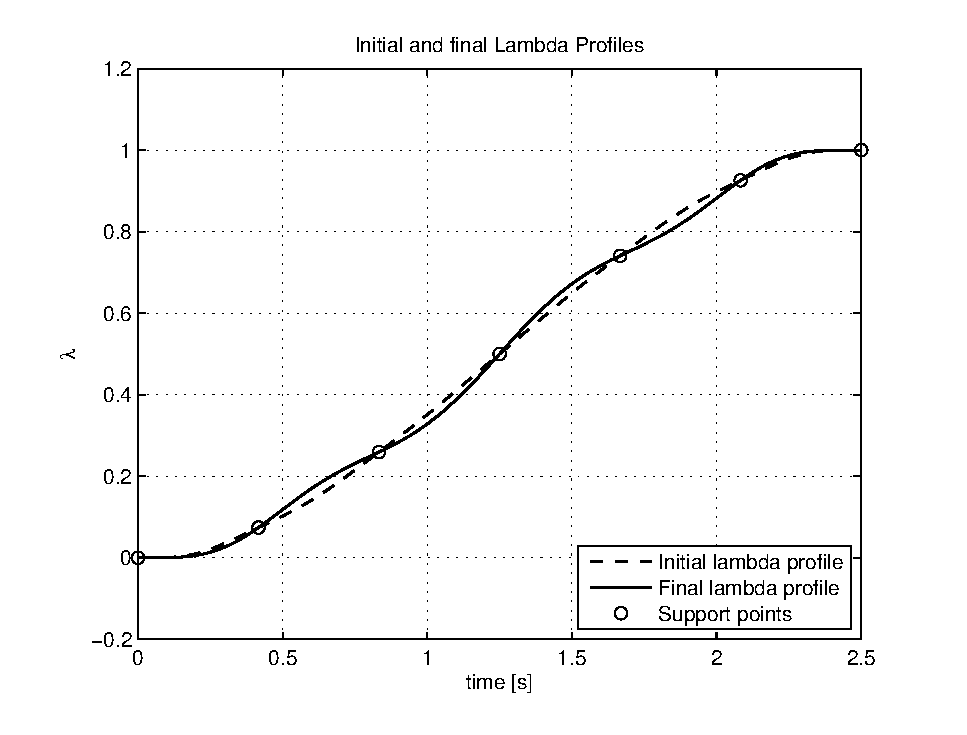
\includegraphics[scale=0.5]{lambda.eps}
\caption{Motion profile for a wave trajectory}
\label{Lambda profile}
\end{figure}

In Figure \ref{Quadrocopter} is shown a schematic drawing of a quadrocopter, taken from \cite{ILC_Angela}.

\begin{figure}
\center		
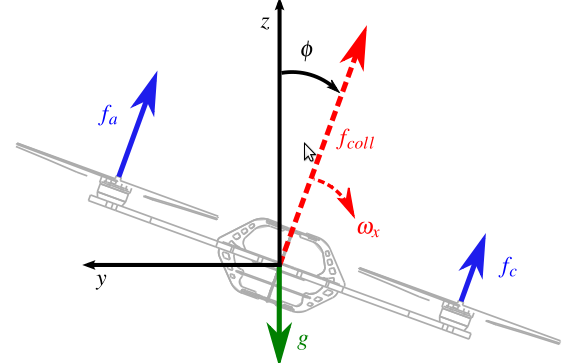
\includegraphics[scale=0.4]{quad.png}
\caption{A 2D schematic drawing of a quadrocopter}
\label{Quadrocopter}
\end{figure}


\end{document}